
%%%%%%%%%%%%%%%%%%%%%%%%%%%%%%%%%%%%%%%%%%%%%%%%%%%%%%%%%%%%%%%%%%%%%%%%%%%%%%%%
%
% Analysis and Plotting
%
%%%%%%%%%%%%%%%%%%%%%%%%%%%%%%%%%%%%%%%%%%%%%%%%%%%%%%%%%%%%%%%%%%%%%%%%%%%%%%%%

\section{Analysis}
\label{sec:analysis}

%%%%%%%%%%%%%%%%%%%%%%%%%%%%%%%%%%%%%%%%%%%%%%%%%%%%%%%%%%%%%%%%%%%%%%%%%%%%%%%%


In this section, we discuss the details of the pipeline used for this work, including the analysis and plotting codes, databases, and automation scripts.  We also present an overview of the results obtained at each step.  A more in depth discussion of the observed trends and interpretations of results are presented in Sections~\ref{sec:2lpt--results} and \ref{sec:2lpt--discussion}.

As a high-level overview, we gather snapshots from previously run \lpt\ and \za\ simulations, find halos in each snapshot with \rockstar, match halos between simulations with \crossmatch, and compare the differences in various properties between corresponding \lpt\ and \za\ halos, primarily as functions of redshift and halo mass.  The specific codes developed for and used in our analysis are provided in the Appendices, and are referenced with the relevant discussions below.




%~~~~~~~~~~~~~~~~~~~~~~~~~~~~~~~~~~~~~~~~~~~~~~~~~~~~~~~~~~~~~~~~~~~~~~~~~~~~~~~
\subsection{Halo Properties}
\label{subsec:analysis--halo_properties}
%~~~~~~~~~~~~~~~~~~~~~~~~~~~~~~~~~~~~~~~~~~~~~~~~~~~~~~~~~~~~~~~~~~~~~~~~~~~~~~~


Halos are identified and measured with the \rockstar\ halo finder (see Section~\ref{sec:rockstar} for implementation details).

Text goes here.



%:::::::::::::::::::::::::::::::::::::::::::::::::::::::::::::::::::::::::::::::
\subsubsection{Rockstar Output and Post-processing}
\label{subsubsec:analysis--halo_properties--output}
%:::::::::::::::::::::::::::::::::::::::::::::::::::::::::::::::::::::::::::::::


Text goes here.



%:::::::::::::::::::::::::::::::::::::::::::::::::::::::::::::::::::::::::::::::
\subsubsection{Spherical Overdensity Halo Particles}
\label{subsubsec:analysis--halo_properties--spherical_overdensity}
%:::::::::::::::::::::::::::::::::::::::::::::::::::::::::::::::::::::::::::::::


Text goes here.




%~~~~~~~~~~~~~~~~~~~~~~~~~~~~~~~~~~~~~~~~~~~~~~~~~~~~~~~~~~~~~~~~~~~~~~~~~~~~~~~
\subsection{Density Profile Fitting}
\label{subsec:analysis--profile_fitting}
%~~~~~~~~~~~~~~~~~~~~~~~~~~~~~~~~~~~~~~~~~~~~~~~~~~~~~~~~~~~~~~~~~~~~~~~~~~~~~~~


While \rockstar's output includes measurements for halo virial and scale radii, and thus concentration, we independently fit NFW density profiles to halos and measure concentration as a verification of \rockstar's fitting.  The full density profile python code is presented in Appendix~\ref{app:density_profile}.



%:::::::::::::::::::::::::::::::::::::::::::::::::::::::::::::::::::::::::::::::
\subsubsection{Density Profiles}
\label{subsubsec:analysis--profile_fitting--density_profiles}
%:::::::::::::::::::::::::::::::::::::::::::::::::::::::::::::::::::::::::::::::


For each halo, a list of constituent spherical overdensity particles is obtained from the post-processed BGC2 catalog from \rockstar's output.  For our purposes here, the relevant parameters are particle mass and position.  We also use the values for each halo's center position and virial radius as found by \rockstar.

Density profiles are then constructed by binning the particle positions in logarithmic radial bins from the resolution limit of the simulation to the halo virial radius and multiplying by particle mass.  Before being passed to the fitting routine, density profiles are normalized to unity for both virial radius and maximum density. 



%:::::::::::::::::::::::::::::::::::::::::::::::::::::::::::::::::::::::::::::::
\subsubsection{Fitting}
\label{subsubsec:analysis--profile_fitting--fitting}
%:::::::::::::::::::::::::::::::::::::::::::::::::::::::::::::::::::::::::::::::


Halos are fit using the CurveFit routine from the SciPy Optimize library.  It uses the Levenberg-Marquardt algorithm\cn\ for non-linear least squares fitting.

CurveFit is called by providing a model function, independent variable, measured dependent variable, and optionally weights for the dependent variable and initial guesses for fit coefficients.  Here, our fit function is the NFW dark matter density profile (see Equation~\ref{eq:nfw_profile}).  The free parameters to be fit are the scale radius $R_{s}$ and the characteristic density $\rho_{0}$.

As the least squares algorithm is sensitive to local minima, care must be taken in choosing initial guesses for the fit coefficients.  Additionally, large dynamic range in the fit parameters tended to produce poor results.  We explored a number of solutions to improve solution stability, including fitting in logarithmic space and randomizing the initial guesses and picking the best solution.  We found the best results were achieved by normalizing the data to unity for both radius and density, and choosing initial guesses within an order of magnitude for a typical halo, namely, normalized $R_{s} = 0.1$ and normalized $\rho_{0} = 1.0$.

Some halos with irregular profiles presented the problem of the fitting algorithm choosing an unphysical scale radius larger than the virial radius of the halo.  In order to heavily penalize this option from being chosen by the fitting algorithm, the dependent variable returned by the model function must differ from the input measured dependent variable as much as possible.  However, we discovered that the transition must also be smooth, as a disjointed jump such as, say, returning a very large number for every value if $R_{s} > R_{\mathrm{vir}}$ would cause the algorithm to fail.  We achieve this smooth transition penalty by adding the term $(R_{s} - 1) e^{r}$ to the density returned by the model function if the fitting algorithm tries to guess a value of $R_{s}$ larger than $R_{\mathrm{vir}}$.  However, while this did force halos to have definable concentrations, these halos often ended up with best fit scale radii equal to or just slightly less than the virial radii.

As we fit halos over a large range in redshift, we found low particle count halos to have noisy density profiles that were inherently more difficult to properly fit.  Throughout our analysis, we use a lower bound of 100 particles to define a halo.  At high redshift, even the largest halos are just beginning to cross this threshold.  With such few particles spread across the number of bins necessary to properly define a density profile, we are left with only a handful of particles per bin.  In Figure~\ref{fig:fitting--density_profiles}, we compare one of the largest halos at $z = 14$ with one of the largest halos at the end of the simulation at $z = 6$.

\begin{figure}[t]
	\centering
	\begin{subfigure}{}
		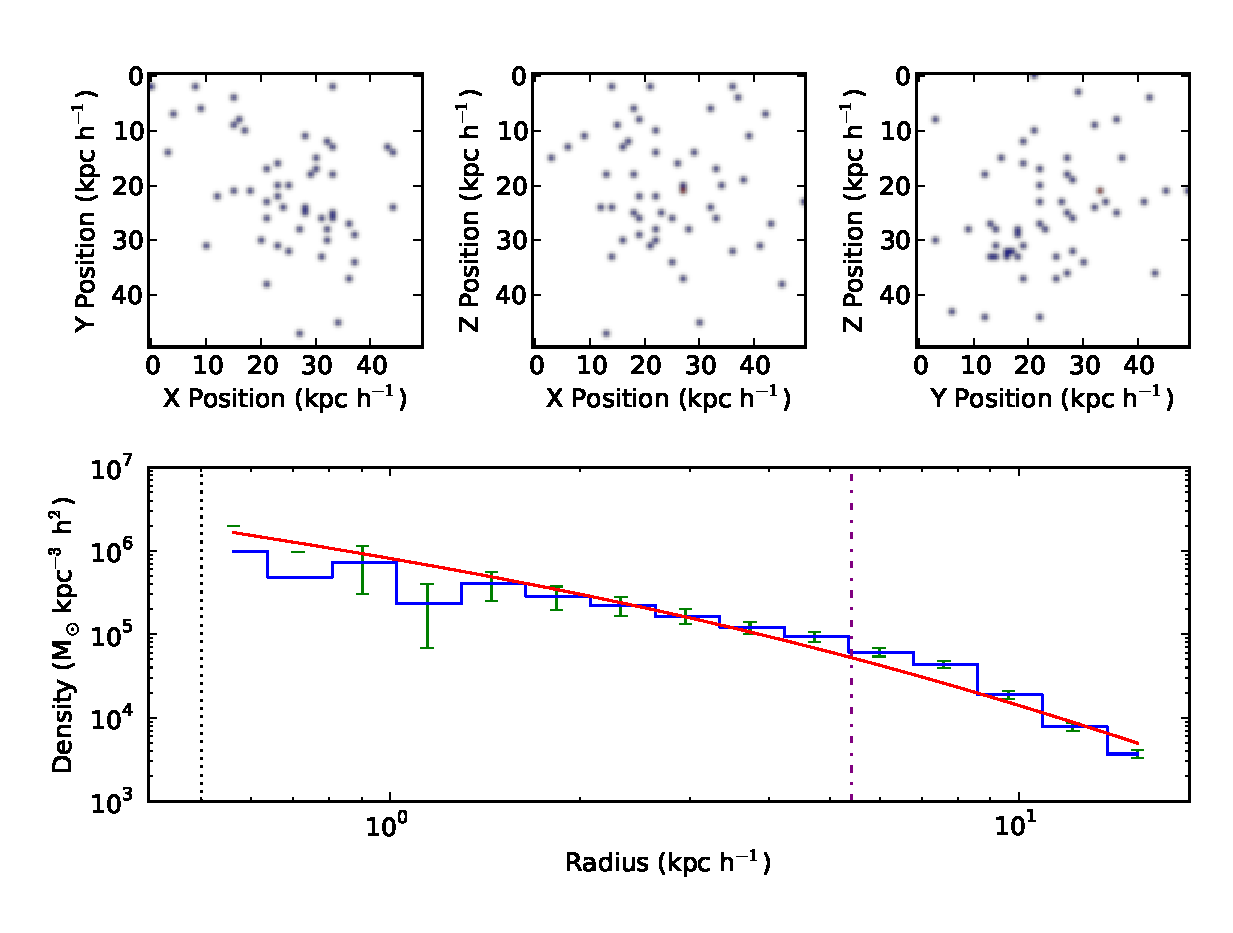
\includegraphics[width=0.75\linewidth]{analysis/2lpt_040_density_profile_0.eps}
	\end{subfigure}
	\\
	\begin{subfigure}{}
		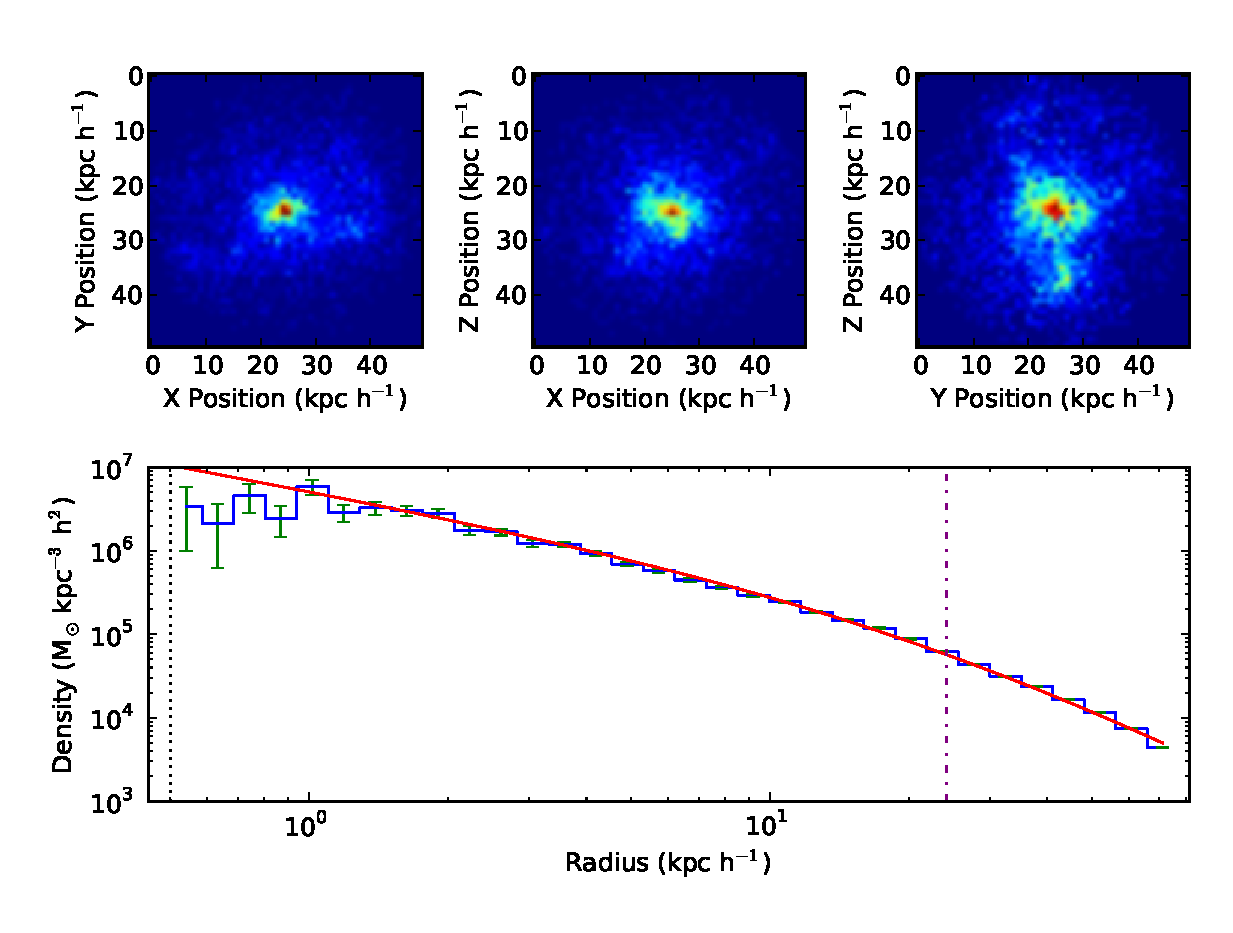
\includegraphics[width=0.75\linewidth]{analysis/2lpt_061_density_profile_0.eps}
	\end{subfigure}
	\caption[Density profiles for two large halos at $z = 14$ and $z = 6$.]{\footnotesize Density profiles for two large halos at $z = 14$ and $z = 6$.  Both halos are from the Box 1 \lpt\ simulation, and are the largest halos at their respective redshifts.  \mrk{(Get rid of density projections.)}}
	\label{fig:fitting--density_profiles}
\end{figure}



%:::::::::::::::::::::::::::::::::::::::::::::::::::::::::::::::::::::::::::::::
\subsubsection{Characterization of Uncertainty}
\label{subsubsec:analysis--profile_fitting--uncertainty}
%:::::::::::::::::::::::::::::::::::::::::::::::::::::::::::::::::::::::::::::::


An initial motivation for finding our own concentration parameters independent from \rockstar\ is that \rockstar\ does not provide information about the quality of its density profile fits.  We assign Poisson errors to the density in each bin such that $\sigma_{\rho} = \rho \sqrt{N} / N$, where $\rho$ is the density and $N$ is the number of particles in each bin.  These uncertainties are then provided as weights to the CurveFit routine.  Upon finding a best fit, the routine provides the fit parameters and an estimation of the uncertainty in those parameters via a covariance matrix, which we use to uncertainty in the concentration.  Additionally, we find the $\chi^{2}$ for the overall fit, which we use as an indicator of whether to accept or reject the fit for a given halo.



%:::::::::::::::::::::::::::::::::::::::::::::::::::::::::::::::::::::::::::::::
\subsubsection{Mass Profiles}
\label{subsubsec:analysis--profile_fitting--mass_profiles}
%:::::::::::::::::::::::::::::::::::::::::::::::::::::::::::::::::::::::::::::::


Text goes here.  Mass profiles tested to avoid binning issues and the stats stuff Manodeep learned at the conference.  Bad fitting results, so abandoned.  Figure~\ref{fig:mass_profile}.

\begin{figure}[t]
	\centering
	\begin{subfigure}{}
		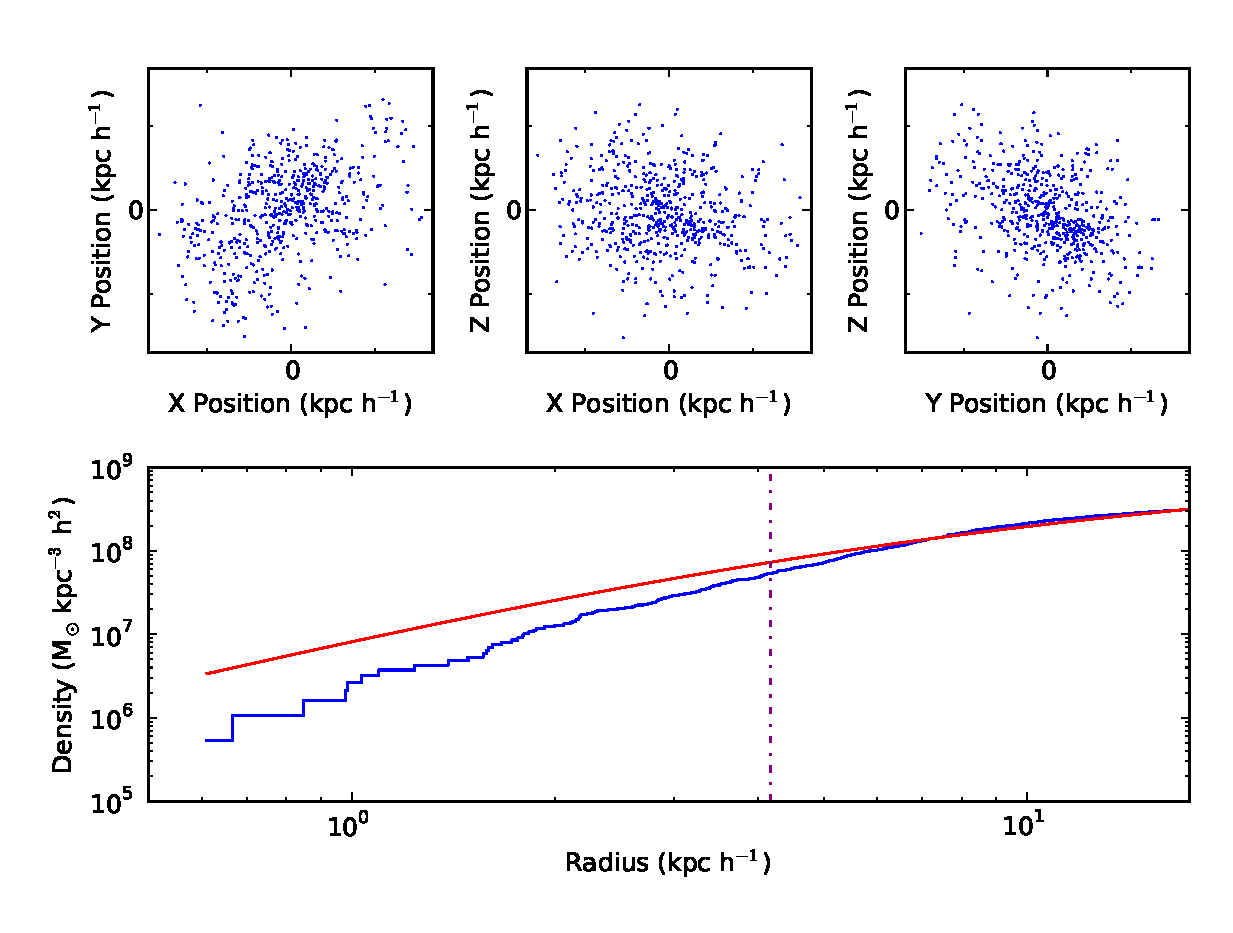
\includegraphics[width=0.75\linewidth]{analysis/2lpt_061_mass_profile_0.eps}
	\end{subfigure}
	\caption[Mass profiles a large halo at $z = 6$.]{\footnotesize Mass profiles for a large halo at $z = 6$.  \mrk{(Get rid of density projections.)}}
	\label{fig:mass_profile}
\end{figure}



%:::::::::::::::::::::::::::::::::::::::::::::::::::::::::::::::::::::::::::::::
\subsubsection{Concentration Comparison to \rockstar}
\label{subsubsec:analysis--profile_fitting--rockstar_comparison}
%:::::::::::::::::::::::::::::::::::::::::::::::::::::::::::::::::::::::::::::::


Overall, we do not find good agreement with \rockstar.  Using a script (see Appendix~\ref{app:concentration_comparison}) to compare the concentrations derived from our fits with those from \rockstar.  At $z = 6$, we find that only 26\% of halos fit by our method have concentrations within 20\% of concentrations as measured by \rockstar.  We have slightly more agreement with high mass halos, with 37\% agreement if we only consider the most massive 10\% of halos.  Additionally, we do not find good fits for every halo.  If the distribution of particles would produce too few bins or the fitting routine exceeded a maximum number of iterations to find a stable solution, the halo is not fit.  We also exclude halos with fits returned with very large $\chi^{2}$ values.  Because of the discrepancies in our results and the fact that we do not find acceptable fits for every halo, we use the more complete \rockstar\ data for the final concentration measurements used in the remainder of our analysis.




%~~~~~~~~~~~~~~~~~~~~~~~~~~~~~~~~~~~~~~~~~~~~~~~~~~~~~~~~~~~~~~~~~~~~~~~~~~~~~~~
\subsection{Cross-matched Halo Catalog}
\label{subsec:analysis--catalog}
%~~~~~~~~~~~~~~~~~~~~~~~~~~~~~~~~~~~~~~~~~~~~~~~~~~~~~~~~~~~~~~~~~~~~~~~~~~~~~~~


With halo catalogs generated by \rockstar\ for both \lpt\ and \za\ simulations, we need to be able to directly compare corresponding halos from the two suites of simulations.  We match halos between simulations based on constituent particles with the \crossmatch\ code modified to import \rockstar's BGC2 binary output files.  Properties of the matched halos are then compiled into one large database per box for further filtering and analysis.



%:::::::::::::::::::::::::::::::::::::::::::::::::::::::::::::::::::::::::::::::
\subsubsection{Cross-matching}
\label{subsubsec:analysis--catalog--crossmatching}
%:::::::::::::::::::::::::::::::::::::::::::::::::::::::::::::::::::::::::::::::


Our simulations are initialized with identical particle ID schemes, and we are thus able to uniquely identify and track matching particles between simulations and match halos based on the largest number of shared particles.  As the full implementation of the \crossmatch\ code is previously discussed in Section~\ref{sec:crossmatch}, we only briefly summarize its place in our analysis pipeline here.  The script in Appendix~\ref{app:crossmatch_setup} sets up the directory structure for the \crossmatch\ analysis and copies the \crossmatch\ parameter files (Appendices~\ref{app:crossmatch_2lpt_config} and \ref{app:crossmatch_za_config}) to the appropriate run directories.  \crossmatch\ is then run for each snapshot via the submission script in Appendix~\ref{app:run_crossmatch}, which is run for each simulation box.

Once caveat of the \crossmatch\ code is that matches are not necessarily unique.  For each halo in the first simulation, only one best match halo will be selected from the second simulation.  However, there may be other halos from the first simulation that also have the same halo from the second simulation selected as a best match.  To counter this, we run \crossmatch\ in both directions---once matching \za\ halos to \lpt\ halos and once matching \lpt\ halos to \za\ halos---and choose best match halos as those that are matched in both directions.  This assures a unique one-to-one matching between \lpt\ and \za\ halos.  The code and submission script that select the best matches from the \lpt-first and \za-first cross-matched halo lists are presented in Appendix~\ref{app:best_match}.



%:::::::::::::::::::::::::::::::::::::::::::::::::::::::::::::::::::::::::::::::
\subsubsection{Database Aggregation and Filtering}
\label{subsubsec:analysis--catalog--aggregation}
%:::::::::::::::::::::::::::::::::::::::::::::::::::::::::::::::::::::::::::::::


We now have raw halo data we need for further study, but are also left with a large number of disparate files that contain this information.  For every snapshot, we have cross-simulation halo matching information from \crossmatch\ and the best match selection script, independent density profile and concentration measurement information from the density profile program, and original halo properties and host halo membership information from \rockstar\ spread across plaintext and BGC2 binary files for each processor on which \rockstar\ was run, all for three simulation boxes each for both \lpt\ and \za.

We combine the information from all of these file into one centralized database per snapshot with the database generation program and submission script in Appendix~\ref{app:database_generation}.  The program reads in all of the source data files, finds companion halos from the output of \crossmatch, and outputs all available data for each halo pair aggregated together.  The program is run for each of our 62 snapshots per simulation box, giving 186 total database files.

With the first version of our database generation code, total runtime became a significant factor.  The halo matching code was initially implemented in a naive double loop search through all the data files to find collect halo pair properties.  Pure python loop structures are exceedingly slow for larger data sets, and an initial estimate gave a runtime on the order of weeks or months.  This was unacceptable, as there are many snapshots, and the aggregation may need to be performed multiple times if any of the previous steps in the analysis pipeline were to be modified.  The code was therefore rewritten to take full advantage of the vectorization of the NumPy library, achieving a massive speedup to a runtime of order a few seconds.

In order to retain a centralized database of all available information for matched halos, we do not filter out halos at this step.  Subsequent analysis, however, does remove halo pairs from consideration in certain circumstances.  For early analysis involving our independent density profile fitting, we remove halos based on evidence of a poor fit, including halos that have measured concentrations greater than 100 or less than 1, $\rho_{0}$ less than zero, or $\chi^{2}$ greater than 10.  For all analysis, we remove halos with fewer than 100 particles and halos that exist as substructure in a larger host halo.




%~~~~~~~~~~~~~~~~~~~~~~~~~~~~~~~~~~~~~~~~~~~~~~~~~~~~~~~~~~~~~~~~~~~~~~~~~~~~~~~
\subsection{Halo Comparison}
\label{subsec:analysis--halo_comparison}
%~~~~~~~~~~~~~~~~~~~~~~~~~~~~~~~~~~~~~~~~~~~~~~~~~~~~~~~~~~~~~~~~~~~~~~~~~~~~~~~


Text goes here.



%:::::::::::::::::::::::::::::::::::::::::::::::::::::::::::::::::::::::::::::::
\subsubsection{Match Verification}
\label{subsubsec:analysis--halo_comparison--match_verification}
%:::::::::::::::::::::::::::::::::::::::::::::::::::::::::::::::::::::::::::::::


Text goes here.



%:::::::::::::::::::::::::::::::::::::::::::::::::::::::::::::::::::::::::::::::
\subsubsection{Morphology}
\label{subsubsec:analysis--halo_comparison--morphology}
%:::::::::::::::::::::::::::::::::::::::::::::::::::::::::::::::::::::::::::::::


Text goes here.



%:::::::::::::::::::::::::::::::::::::::::::::::::::::::::::::::::::::::::::::::
\subsubsection{Density Profiles}
\label{subsubsec:analysis--halo_comparison--density_profiles}
%:::::::::::::::::::::::::::::::::::::::::::::::::::::::::::::::::::::::::::::::


Text goes here.




%~~~~~~~~~~~~~~~~~~~~~~~~~~~~~~~~~~~~~~~~~~~~~~~~~~~~~~~~~~~~~~~~~~~~~~~~~~~~~~~
\subsection{Difference Distributions}
\label{subsec:analysis--difference_histograms}
%~~~~~~~~~~~~~~~~~~~~~~~~~~~~~~~~~~~~~~~~~~~~~~~~~~~~~~~~~~~~~~~~~~~~~~~~~~~~~~~


Text goes here.



%:::::::::::::::::::::::::::::::::::::::::::::::::::::::::::::::::::::::::::::::
\subsubsection{Histograms}
\label{subsubsec:analysis--difference_histograms--binning}
%:::::::::::::::::::::::::::::::::::::::::::::::::::::::::::::::::::::::::::::::


Text goes here.



%:::::::::::::::::::::::::::::::::::::::::::::::::::::::::::::::::::::::::::::::
\subsubsection{Fitting}
\label{subsubsec:analysis--difference_histograms--fitting}
%:::::::::::::::::::::::::::::::::::::::::::::::::::::::::::::::::::::::::::::::


Text goes here.
% Model functions
% Initial guesses
% Fit coefficients



%:::::::::::::::::::::::::::::::::::::::::::::::::::::::::::::::::::::::::::::::
\subsubsection{Mass Quartiles}
\label{subsubsec:analysis--difference_histograms--mass_quartiles}
%:::::::::::::::::::::::::::::::::::::::::::::::::::::::::::::::::::::::::::::::


Text goes here.




%~~~~~~~~~~~~~~~~~~~~~~~~~~~~~~~~~~~~~~~~~~~~~~~~~~~~~~~~~~~~~~~~~~~~~~~~~~~~~~~
\subsection{Redshift Trends}
\label{subsec:analysis--redshift_trends}
%~~~~~~~~~~~~~~~~~~~~~~~~~~~~~~~~~~~~~~~~~~~~~~~~~~~~~~~~~~~~~~~~~~~~~~~~~~~~~~~


Text goes here.



%:::::::::::::::::::::::::::::::::::::::::::::::::::::::::::::::::::::::::::::::
\subsubsection{Mean and Standard Deviation}
\label{subsubsec:analysis--redshift_trends--mean_stdev}
%:::::::::::::::::::::::::::::::::::::::::::::::::::::::::::::::::::::::::::::::


Text goes here.



%:::::::::::::::::::::::::::::::::::::::::::::::::::::::::::::::::::::::::::::::
\subsubsection{Skew}
\label{subsubsec:analysis--redshift_trends--skew}
%:::::::::::::::::::::::::::::::::::::::::::::::::::::::::::::::::::::::::::::::


Text goes here.



%:::::::::::::::::::::::::::::::::::::::::::::::::::::::::::::::::::::::::::::::
\subsubsection{Kurtosis}
\label{subsubsec:analysis--redshift_trends--kurtosis}
%:::::::::::::::::::::::::::::::::::::::::::::::::::::::::::::::::::::::::::::::


Text goes here.

The standard deviation of a function $f(x_{1},x_{2},\dots,x_{n})$ is, in general, given by
\begin{equation} \label{eq:general_stdev}
	s_{f} = \sqrt{\sum_{x} \left( \frac{\partial f}{\partial x} \right)^{2} s_{x}^{2}}
\end{equation}
with summation over all independent variables $x$.  The generalized normal distribution
\begin{equation} \label{eq:generalized_normal}
	f(x) = \frac{\beta}{2 \alpha \Gamma(1/\beta)} e^{-(|x - \mu| / \alpha)^{\beta}}
\end{equation}
with mean $\mu$, scale parameter $\alpha$, and shape parameter $\beta$, has excess kurtosis
\begin{equation} \label{eq:kurtosis}
	\gamma_{2} = \frac{\Gamma(5/\beta) \Gamma(1/\beta)}{\Gamma(3/\beta)^{2}} - 3.
\end{equation}
The gamma function
\begin{equation} \label{eq:gamma_function}
	\Gamma(x) = \int_{0}^{\infty} t^{x-1} e^{-t} \dd t
\end{equation}
has the first derivative
\begin{equation} \label{eq:gamma_prime}
	\Gamma'(x) = \Gamma(x) \psi_{0}(x)
\end{equation}
where the digamma function $\digamma$ is the derivative of the logarithm of the gamma function and is given by
\begin{equation} \label{eq:digamma}
	\digamma(x) = \int_{0}^{\infty} \left( \frac{e^{-t}}{t} - \frac{e^{-xt}}{1 - e^{-t}} \right) \dd t
\end{equation}
if the real part of $x$ is positive.

We now apply \eqref{eq:general_stdev} to \eqref{eq:kurtosis} to find the standard deviation of the excess kurtosis:
\begin{align} \label{eq:kurt_err_partial1}
	s_{\gamma_{2}} &= \sqrt{ \left( \frac{\diff \gamma_{2}}{\diff \beta} \right)^{2} s_{\beta}^{2} } \\
		&= s_{\beta} \frac{\diff \gamma_{2}}{\diff \beta} \\
		&= s_{\beta} \frac{\diff}{\diff \beta} \left[ \frac{\Gamma(5/\beta) \Gamma(1/\beta)}{\Gamma(3/\beta)^{2}} - 3 \right].
\end{align}
Making the substitution $x = 1 / \beta$ and $\diff x = - 1 / \beta^{2} \dd \beta$, taking the derivative, and doing a bit of algebra, we have:
\begin{align} \label{eq:kurt_err_partial2}
	s_{\gamma_{2}} &= s_{\beta} \frac{\diff \gamma_{2}}{\diff x} \frac{\diff x}{\diff \beta} \\
		&= s_{\beta} \left( -\frac{1}{\beta^{2}} \right) \frac{\diff}{\diff x} \left[ \frac{\Gamma(5x) \Gamma(x)}{\Gamma(3x)} - 3 \right] \\
		&= -s_{\beta} x^{2} \left\{ \frac{\Gamma(3x)^{2} \frac{\diff}{\diff x} [\Gamma(5x) \Gamma(x)] - \Gamma(5x) \Gamma(x) \frac{\diff}{\diff x} [\Gamma(3x)^{2}]}{\Gamma(3x)^{4}} \right\} \\
		&= -s_{\beta} \frac{x^{2}}{\Gamma(3x)^{4}} \left\{ \Gamma(3x)^{2} [5\Gamma(5x) \digamma(5x) \Gamma(x) + \Gamma(5x) \Gamma(x) \digamma(x)] - \Gamma(5x) \Gamma(x) [6\Gamma(3x)^{2} \digamma(3x)] \right\} \\
		&= s_{\beta} \frac{x^{2}}{\Gamma(3x)^{4}} \left\{ 6\Gamma(5x) \Gamma(3x)^{2} \Gamma(x) \digamma(3x) - \Gamma(5x) \Gamma(3x)^{2} \Gamma(x) [5\digamma(5x) + \digamma(x)] \right\} \\
		&= s_{\beta} \frac{x^{2}}{\Gamma(3x)^{4}} \left\{ \Gamma(5x) \Gamma(3x)^{2} \Gamma(x) [6\digamma(3x) - 5\digamma(5x) - \digamma(x)] \right\} \\
		&= s_{\beta} x^{2} \frac{\Gamma(5x) \Gamma(x)}{\Gamma(3x)^{2}} [6\digamma(3x) - 5\digamma(5x) - \digamma(x)].
\end{align}
Substituting back in for $x$ and recognizing an occurance of $\gamma_{2}$, we have the result
\begin{equation} \label{eq:kurt_err}
	s_{\gamma_{2}} = s_{\beta} \frac{1}{\beta^{2}} \left( \gamma_{2} + 3 \right) \left[ 6 \digamma(3/\beta) - 5 \digamma(5/\beta) - \digamma(1/\beta) \right]
\end{equation}
with which we can find the uncertainty in the kurtosis given the value and uncertainty of the shape parameter $\beta$.




%~~~~~~~~~~~~~~~~~~~~~~~~~~~~~~~~~~~~~~~~~~~~~~~~~~~~~~~~~~~~~~~~~~~~~~~~~~~~~~~
\subsection{2-D Histograms}
\label{subsec:analysis--2d_histograms}
%~~~~~~~~~~~~~~~~~~~~~~~~~~~~~~~~~~~~~~~~~~~~~~~~~~~~~~~~~~~~~~~~~~~~~~~~~~~~~~~


Text goes here.



%:::::::::::::::::::::::::::::::::::::::::::::::::::::::::::::::::::::::::::::::
\subsubsection{Binning and Plotting}
\label{subsubsec:analysis--2d_histograms--binning_plotting}
%:::::::::::::::::::::::::::::::::::::::::::::::::::::::::::::::::::::::::::::::


Text goes here.



%:::::::::::::::::::::::::::::::::::::::::::::::::::::::::::::::::::::::::::::::
\subsubsection{Fitting}
\label{subsubsec:analysis--2d_histograms--fitting}
%:::::::::::::::::::::::::::::::::::::::::::::::::::::::::::::::::::::::::::::::


Text goes here.




%~~~~~~~~~~~~~~~~~~~~~~~~~~~~~~~~~~~~~~~~~~~~~~~~~~~~~~~~~~~~~~~~~~~~~~~~~~~~~~~
\subsection{Alternate Difference Distributions}
\label{subsec:analysis--alt_diff_dist}
%~~~~~~~~~~~~~~~~~~~~~~~~~~~~~~~~~~~~~~~~~~~~~~~~~~~~~~~~~~~~~~~~~~~~~~~~~~~~~~~


Text goes here.



%:::::::::::::::::::::::::::::::::::::::::::::::::::::::::::::::::::::::::::::::
\subsubsection{Equivalent Displacement}
\label{subsubsec:analysis--alt_diff_dist--equiv_displacment}
%:::::::::::::::::::::::::::::::::::::::::::::::::::::::::::::::::::::::::::::::


Text goes here.



%:::::::::::::::::::::::::::::::::::::::::::::::::::::::::::::::::::::::::::::::
\subsubsection{Redshift Trends}
\label{subsubsec:analysis--alt_diff_dist--trends}
%:::::::::::::::::::::::::::::::::::::::::::::::::::::::::::::::::::::::::::::::


Text goes here.




